

\tikzset{every picture/.style={line width=0.75pt}} %set default line width to 0.75pt        

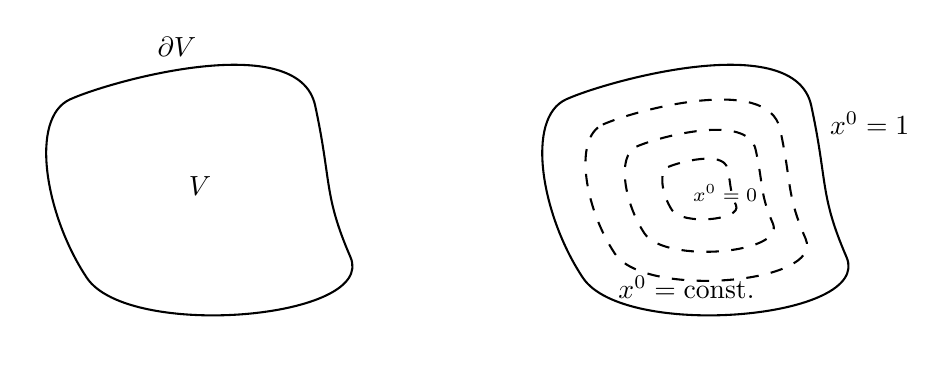
\begin{tikzpicture}[x=0.75pt,y=0.75pt,yscale=-1,xscale=1]
	%uncomment if require: \path (0,151); %set diagram left start at 0, and has height of 151
	
	%Shape: Polygon Curved [id:ds3297526743622252] 
	\draw   (132.37,38.39) .. controls (152.37,29.39) and (242.37,4.39) .. (250.37,41.39) .. controls (258.37,78.39) and (254.37,84.39) .. (267.37,114.39) .. controls (280.37,144.39) and (160.37,154.39) .. (140.37,124.39) .. controls (120.37,94.39) and (112.37,47.39) .. (132.37,38.39) -- cycle ;
	%Shape: Polygon Curved [id:ds46432420576579103] 
	\draw   (371.37,38.39) .. controls (391.37,29.39) and (481.37,4.39) .. (489.37,41.39) .. controls (497.37,78.39) and (493.37,84.39) .. (506.37,114.39) .. controls (519.37,144.39) and (399.37,154.39) .. (379.37,124.39) .. controls (359.37,94.39) and (351.37,47.39) .. (371.37,38.39) -- cycle ;
	%Shape: Polygon Curved [id:ds7205956003748912] 
	\draw  [dash pattern={on 4.5pt off 4.5pt}] (388.99,50.55) .. controls (403.46,44.03) and (468.57,25.95) .. (474.36,52.72) .. controls (480.14,79.48) and (477.25,83.82) .. (486.66,105.53) .. controls (496.06,127.23) and (409.25,134.46) .. (394.78,112.76) .. controls (380.31,91.06) and (374.52,57.06) .. (388.99,50.55) -- cycle ;
	%Shape: Polygon Curved [id:ds031201153637908652] 
	\draw  [dash pattern={on 4.5pt off 4.5pt}] (405.18,61.2) .. controls (414.91,56.82) and (458.72,44.65) .. (462.61,62.66) .. controls (466.51,80.67) and (464.56,83.59) .. (470.89,98.19) .. controls (477.21,112.79) and (418.81,117.66) .. (409.07,103.05) .. controls (399.34,88.45) and (395.45,65.58) .. (405.18,61.2) -- cycle ;
	%Shape: Polygon Curved [id:ds9615417238944546] 
	\draw  [dash pattern={on 4.5pt off 4.5pt}] (420.42,71.01) .. controls (425.26,68.83) and (447.07,62.78) .. (449.01,71.74) .. controls (450.95,80.71) and (449.98,82.16) .. (453.13,89.43) .. controls (456.28,96.7) and (427.2,99.12) .. (422.35,91.85) .. controls (417.51,84.58) and (415.57,73.19) .. (420.42,71.01) -- cycle ;
	
	% Text Node
	\draw (188,74) node [anchor=north west][inner sep=0.75pt]    {$\mathscr{V}$};
	% Text Node
	\draw (173,7) node [anchor=north west][inner sep=0.75pt]    {$\partial \mathscr{V}$};
	% Text Node
	\draw (497,43) node [anchor=north west][inner sep=0.75pt]    {$x^{0} =1$};
	% Text Node
	\draw (395,122) node [anchor=north west][inner sep=0.75pt]    {$x^{0} =\mathrm{const.}$};
	% Text Node
	\draw (431,78) node [anchor=north west][inner sep=0.75pt]  [font=\scriptsize]  {$x^{0} =0$};
	
	
\end{tikzpicture}